\documentclass[12pt]{article}

\usepackage[margin=1in]{geometry}
\usepackage{amsmath,amsthm,amssymb}
\usepackage{nccmath}
\usepackage{mathtools}
\usepackage{mathrsfs}
\usepackage{enumitem}
\usepackage{physics}
\usepackage{tensor}
\usepackage{subcaption}
\usepackage{pdfpages}
\usepackage{graphicx}
\graphicspath{ {./images/} }

\newcommand{\chrissym}[3]{\Gamma_{#2#3}^#1}

\begin{document}
\title{Homework 6}
\author{Sean Ericson \\ Phys 610}
\maketitle

\section*{Problem 1}
\[ r(\phi) = \frac{a(1-e^2)}{1 + e\cos\phi} \]

\begin{align*}
    x &= r\cos\phi \\
    &= \frac{a(1-e^2)\cos\phi}{1 + e\cos\phi} \\
    y &= r\sin\phi \\
    &= \frac{a(1-e^2)\sin\phi}{1 + e\cos\phi}
\end{align*}
\[ b = a\sqrt{1 - e^2} \]
\[ T^{00} = M\delta(z)\left[\delta(x-x_1)\delta(y-y_1) + \delta(x-x_2)\delta(y-y_2)\right] \]
\begin{align*}
    I_{xx} &= \int\dd^3x\; x^2T^{00} \\
    &= M(x_1^2 + x_2^2) \\
    I_{yy} &= M(y_1^2 + y_2^2)\\
    I_{xy} &= M(x_1y_1 + x_2y_2)
\end{align*}


\section*{Problem 2}
\begin{enumerate}[label=(\alph*)]
    \item First, contracting with the metric we can see that
    \begin{alignat*}{3}
        &\quad & 0 &= \left(G_{\mu\nu} + \Lambda g_{\mu\nu}\right) \\
        &\implies\quad & 0 &= g^{\mu\nu}\left(R_{\mu\nu} - \frac{1}{2}Rg_{\mu\nu} + \Lambda g_{\mu\nu}\right) \\
        &\quad &   &= R - \frac{1}{2}4R + 4\Lambda \\
        &\implies\quad & R &= 4\Lambda.
    \end{alignat*}
    Then,
    \begin{alignat*}{3}
        &\quad & 0 &= R_{\mu\nu} - \frac{1}{2}Rg_{\mu\nu} + \Lambda g_{\mu\nu} \\
        &\quad &   &= R_{\mu\nu} - \Lambda g_{\mu\nu}
    \end{alignat*}
    Assuming the general form for the line element (as in Carrol)
    \[ \dd s^2 = -e^{2\alpha(r)}\dd t^2 + e^{2\beta(r)}\dd r^2 + r^2\left(\dd\theta^2 + \sin^2\theta\dd\phi^2\right), \]
    the non-zero components of the Ricci tensor are
    \begin{align*}
        R_{tt} &= e^{2(\alpha-\beta)}\left(\frac{2}{r}\alpha' + \alpha'^2 + \alpha''\right) \\
        R_{rr} &= \frac{2}{r}\beta' + \alpha'\beta' -  \alpha'^2 - \alpha'' \\
        R_{\theta\theta} &= e^{-2\beta}\left(r\beta' - r\alpha'\right) + 1 \\
        R_{\phi\phi} &= \sin^2\theta\left(e^{-2\beta}\left(\left(r\beta' - r\alpha'\right) -1\right) + 1 + r^2\right).
    \end{align*}
    The Einstein equation then gives
    \begin{align*}
        0 &= e^{2(\alpha-\beta)}\left(\frac{2}{r}\alpha' + \alpha'^2 + \alpha''\right) - \Lambda e^{2\alpha} \\
        0 &= \frac{2}{r}\beta' + \alpha'\beta' -  \alpha'^2 - \alpha'' + \Lambda e^{2\beta} \\
        0 &= e^{-2\beta}\left(\left(r\beta' - r\alpha'\right) -1\right) + 1 + \Lambda r^2 \\
        0 &= \sin^2\theta\left(e^{-2\beta}\left(\left(r\beta' - r\alpha'\right) -1\right) + 1 + \Lambda r^2\right).
    \end{align*}
    Multiplying the first equation by $e^{-2\alpha}$, the second by $e^{-2\beta}$, then adding gives
    \begin{alignat*}{3}
        &\quad & 0 &= e^{-2\beta}\left(\frac{2}{r}\alpha' + \alpha'^2 + \alpha''\right) - \Lambda + e^{-2\beta}\left(\frac{2}{r}\beta' + \alpha'\beta' -  \alpha'^2 - \alpha''\right) + \Lambda \\
        &\quad &   &= \frac{2}{r}\left(\alpha' + \beta'\right) \\
        &\implies\quad & \alpha' &= -\beta' \\
        &\implies\quad & \alpha(r) &= -\beta(r) + c.
    \end{alignat*}
    However, we can set $c = 0$ by taking $t \to e^{-c}t$. The third of the Einstein equations is now
    \begin{alignat*}{3}
        &\quad & 0 &= e^{-2\beta}\left(\left(r\beta' - r\alpha'\right) -1\right) + 1 + \Lambda r^2 \\
        &\quad &   &= e^{2\alpha}\left(-2r\alpha' - 1\right) + 1 + \Lambda r^2 \\
        &\quad &   &= -\partial_r\left(re^{2\alpha}\right) + 1 + \Lambda r^2 \\
        &\implies\quad & \partial_r\left(re^{2\alpha}\right) &= 1 + \Lambda r^2 \\
        &\implies\quad & re^{2\alpha} &= r + \frac{1}{3}\Lambda r^3 + \alpha_0 \\
        &\implies\quad & e^{2\alpha} &= 1 + \frac{1}{3}\Lambda r^2 + \frac{\alpha_0}{r},
    \end{alignat*}
    where $\alpha_0$ is a yet to be determined constant. Plugging this back into the line element, we have
    \[ \dd s^2 = -\left(1 + \frac{\alpha_0}{r} + \frac{1}{3}\Lambda r^2\right)\dd t^2 + \left(1 + \frac{\alpha_0}{r} + \frac{1}{3}\Lambda r^2\right)^{-1}\dd r^2 + r^2\left(\dd\theta^2 + \sin^2\theta\dd\phi^2\right). \]
    Clearly this reduces to the Schwarzschild metric when $\Lambda\to 0$ if we choose $\alpha_0 = -2GM$.

    \item 
    \begin{figure}[h]
        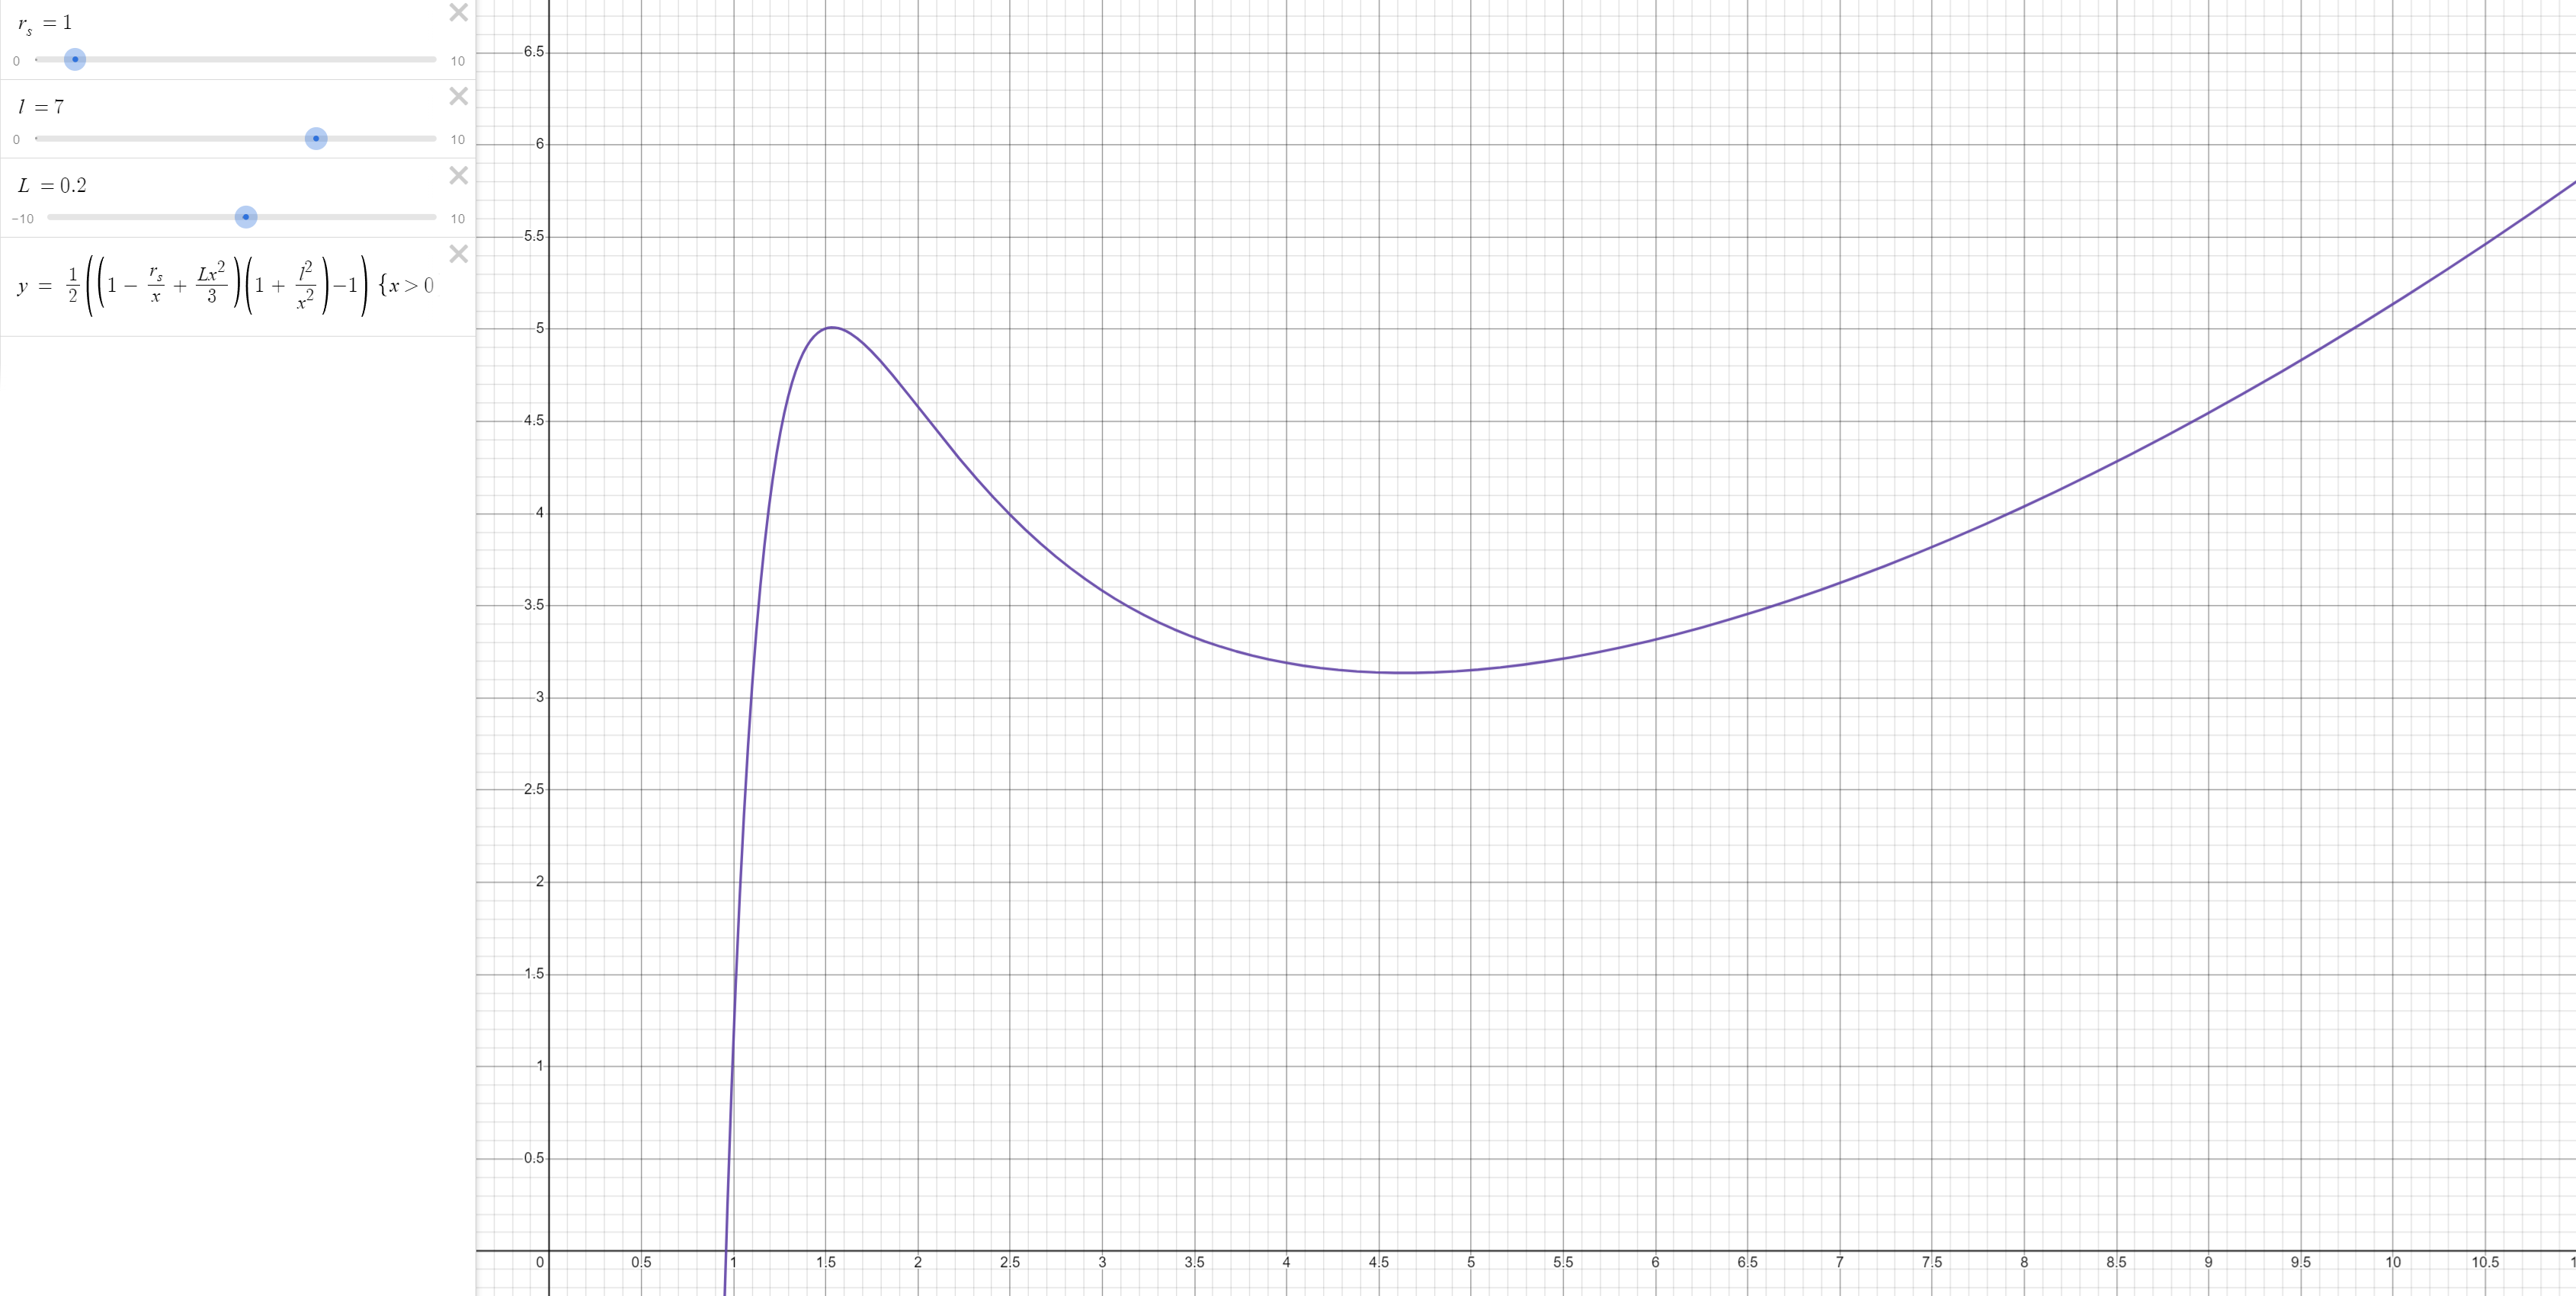
\includegraphics[scale=0.25]{prob2b.PNG}
        \centering
        \caption{$V_\text{eff}(r)$ with $r_s=1$, $l=7$, $\Lambda=0.2$.}
        \label{fig1}
    \end{figure}
    We have the conserved quantities
    \begin{align*}
        e \coloneqq -\xi_t^\mu\dv{x^\mu}{\tau} &= \left(1 - \frac{r_s}{r} + \frac{1}{3}\Lambda r^2\right)\dv{t}{\tau} \\
        l \coloneqq -\xi_\phi^\mu\dv{x^\mu}{\tau} &= -r^2\sin^2\theta\dv{\phi}{\tau}
    \end{align*}

    Normalization of the four-velocity gives
    \begin{alignat*}{3}
        &\quad & \dv{x^\mu}{\tau}\dv{x_\mu}{\tau} &= -1 \\
        &\quad & &= -\left(1 + \frac{r_s}{r} + \frac{1}{3}\Lambda r^2\right)\left(\dv{t}{\tau}\right)^2 + \left(1 + \frac{\alpha_0}{r} + \frac{1}{3}\Lambda r^2\right)^{-1}\left(\dv{r}{\tau}\right)^2 + r^2\left(\dv{\phi}{\tau}\right)^2 \\
        &\quad & &= -e^2\left(1 + \frac{r_s}{r} + \frac{1}{3}\Lambda r^2\right)^{-1} + \left(1 + \frac{\alpha_0}{r} + \frac{1}{3}\Lambda r^2\right)^{-1}\left(\dv{r}{\tau}\right)^2 + \frac{l^2}{r^2} \\
        &\implies\quad & e^2 &= 1 + \frac{r_s}{r} + \frac{1}{3}\Lambda r^2 + \left(\dv{r}{\tau}\right)^2 + \frac{l^2}{r^2}\left(1 + \frac{r_s}{r} + \frac{1}{3}\Lambda r^2\right) \\
        &\quad & &= \left(\dv{r}{\tau}\right)^2 + \left(1 + \frac{r_s}{r} + \frac{1}{3}\Lambda r^2\right)\left(1 + \frac{l^2}{r^2}\right) \\
        &\implies\quad & \mathcal{E} \coloneqq \frac{1}{2}(e^2 - 1) &= \frac{1}{2}\left(\dv{r}{\tau}\right)^2 + V_\text{eff}(r)
    \end{alignat*}
    where
    \begin{align*}
        V_\text{eff}(r) &= \frac{1}{2}\left(\left(1 - \frac{r_s}{r} + \frac{1}{3}\Lambda r^2\right)\left(1 + \frac{l^2}{r^2}\right) - 1\right) \\
        &= \frac{1}{6}\Lambda (r^2 + l^2) - \frac{r_s}{2r} + \frac{l^2}{2r^2} - \frac{r_sl^2}{2r^3}
    \end{align*}
\end{enumerate}


\section*{Problem 3}
\begin{enumerate}[label=(\alph*)]
    \item Calculation done in Mathematica, see Appendix.
    \item The transformation is given by 
    \[ h_{\mu\nu} \to h_{\mu\nu} + \partial_{\mu}\xi_\nu + \partial_nu\xi_\mu \]
    To kill off the $c$s, we need 
    \begin{align*}
        2\partial_0\xi_0 &= -c\sin(k(x-t)), \\
        2\partial_1\xi_1 &= c\sin(k(x-t)), \\
        \partial_0\xi_i &= -\partial_i\xi_0 = 0, \\
        \partial_i\xi_j &= -\partial_j\xi_i = 0 \quad (i,j = y,z).
    \end{align*}
    Integrating, we find that
    \[ \xi_\mu = \mqty(-1\\-1\\0\\0)\frac{c}{2k}\cos(k(x-t)) + b_\mu \]
    where $b_\mu$ is any constant vector. Under this transformation $a$ is unchanged.
\end{enumerate}

\section*{Appendix}
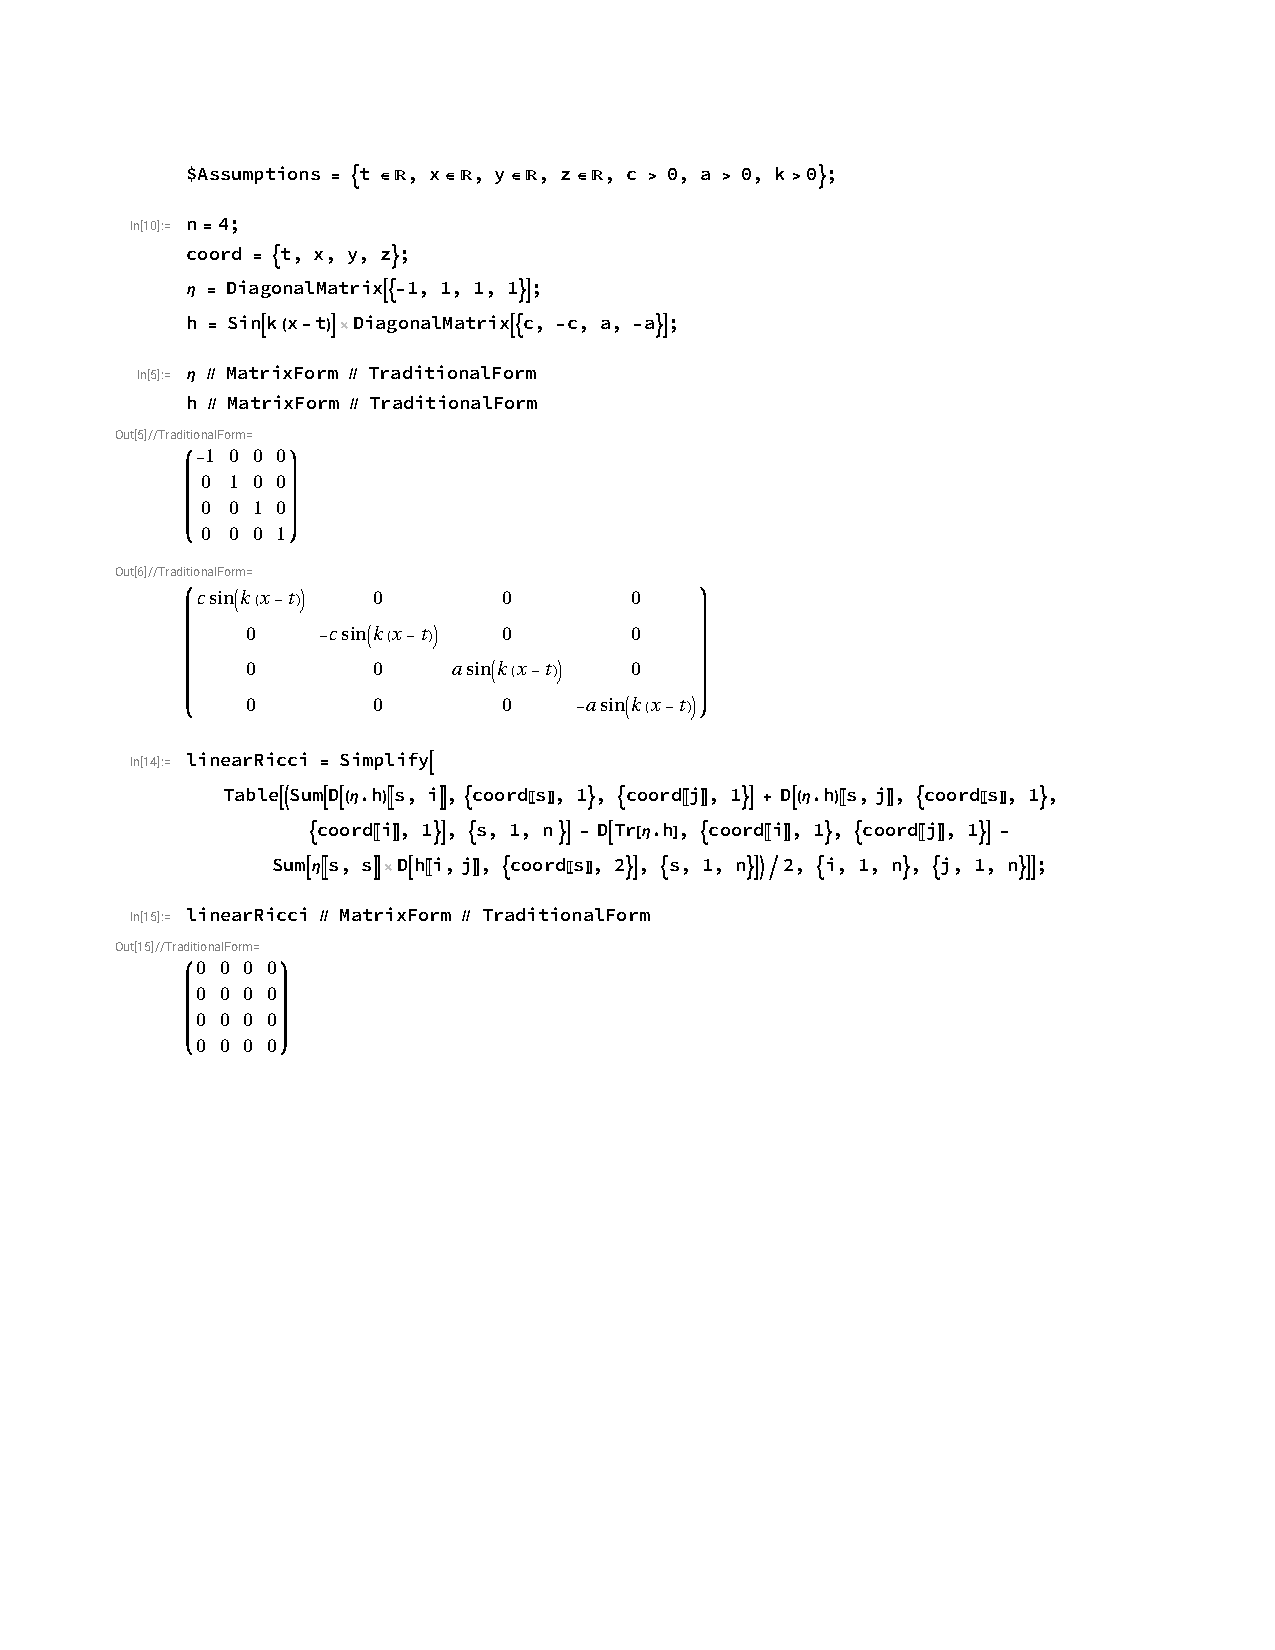
\includepdf[pages=-]{calcs/prob3.pdf}

\end{document}